\documentclass[10pt,a4paper]{article}
\usepackage[utf8]{inputenc}
\usepackage[spanish]{babel}
\usepackage{amsmath}
\usepackage{amsfonts}
\usepackage{amssymb}
\usepackage[T1]{fontenc} 
\usepackage[left=2.00cm, right=2.00cm, top=2.00cm, bottom=2.00cm]{geometry}
\usepackage{acronym}
\usepackage{listings}
\usepackage{graphicx}
\graphicspath{ {images/} }
\usepackage{hyperref}

\usepackage{multirow}
\usepackage[table,xcdraw]{xcolor}

\usepackage[export]{adjustbox}
\usepackage{subcaption}

%%Sobre el código
\usepackage{xcolor}
\usepackage{xparse}
\NewDocumentCommand{\codeword}{v}{%
	\texttt{\textcolor{blue}{#1}}%
}

\setlength{\parindent}{1em}
\setlength{\parskip}{1em}




\title{
Proyecto final\\
\large Visión por Computador \\
}

\author{
Alejandro Alonso Membrilla\\
Alejandro Palencia Blanco\\
}

\date{29/01/2021}



\begin{document}

\maketitle

\newpage

\tableofcontents

\newpage

\section{Introducción}

La creación de conjuntos de datos correctamente etiquetados para el entrenamiento de redes neuronales de forma supervisada es una tarea muy costosa de realizar. Concretamente, en el problema de clasificación de imágenes, esto supone asignar a cada una de las imágenes la etiqueta de la clase a la que pertenece. Alternativamente, en este proyecto estudiamos el aprendizaje autosupervisado como técnica para facilitar el entrenamiento de redes neuronales convolucionales de clasificación de imágenes. Al aplicar este método se parte de conjuntos de datos no etiquetados, los cuales son mucho más fáciles de generar. Normalmente, se suele utilizar una tarea de pretexto que el modelo debe aprender a resolver. A continuación, el modelo preentrenado para resolver dicha tarea puede adaptarse a otro problema que requiera de una extracción de características similar.

Para resolver la tarea de pretexto, previamente es necesario etiquetar los datos a partir de la estructura o características de los mismos y luego entrenar el modelo con el conjunto de datos ya etiquetado de forma supervisada. La clave del aprendizaje autosupervisado es que, al contrario que en aprendizaje supervisado, el proceso de etiquetado necesario para resolver esta tarea es muchísimo menos costoso ya que se realiza de forma automática. 

\subsection{Resolución de puzzles}

Existen varios ejemplos de tareas de pretexto que se pueden utilizar para preentrenar el modelo: colorización de imágenes, resolución de puzzles, ordenación de frames de vídeo, clasificación de imágenes en correctas o corruptas… En este proyecto, tomaremos la resolución de puzzles como nuestra tarea de pretexto.

El problema de la resolución de puzzles consiste en, dada una imagen dividida en un \textit{grid} 3x3 de la que se extraen nueve piezas cuadradas y se desordenan, encontrar la permutación que reordena las piezas y recupera la imagen original. Esta aplicación de aprendizaje autosupervisado ya ha sido estudiada en este \href{https://arxiv.org/pdf/1603.09246v3.pdf}{artículo}, en el cual nos basaremos para el desarrollo de este proyecto. Para resolver esta tarea, sus autores han diseñado una red convolucional con nueve ramas siamesas a la que han puesto el nombre de Context-Free Network (CFN). Cada una de estas ramas es una copia exacta de la red AlexNet (salvo por la primera convolución, que usa un stride de 2 en lugar de 4). Todas ellas comparten todos sus pesos y son las encargadas de procesar cada una de las nueve piezas en las que se particiona la imagen, respectivamente. Después, los vectores de características obtenidos en cada rama se concatenan y se procesan a través de dos capas totalmente conectadas para finalmente llegar al clasificador softmax. Cada una de las posiciones del vector devuelto por el clasificador está asociado a una permutación concreta, luego el objetivo de esta red es devolver un vector con un 1 en la posición correspondiente a la permutación que reordena la imagen.

\begin{figure}[h]
	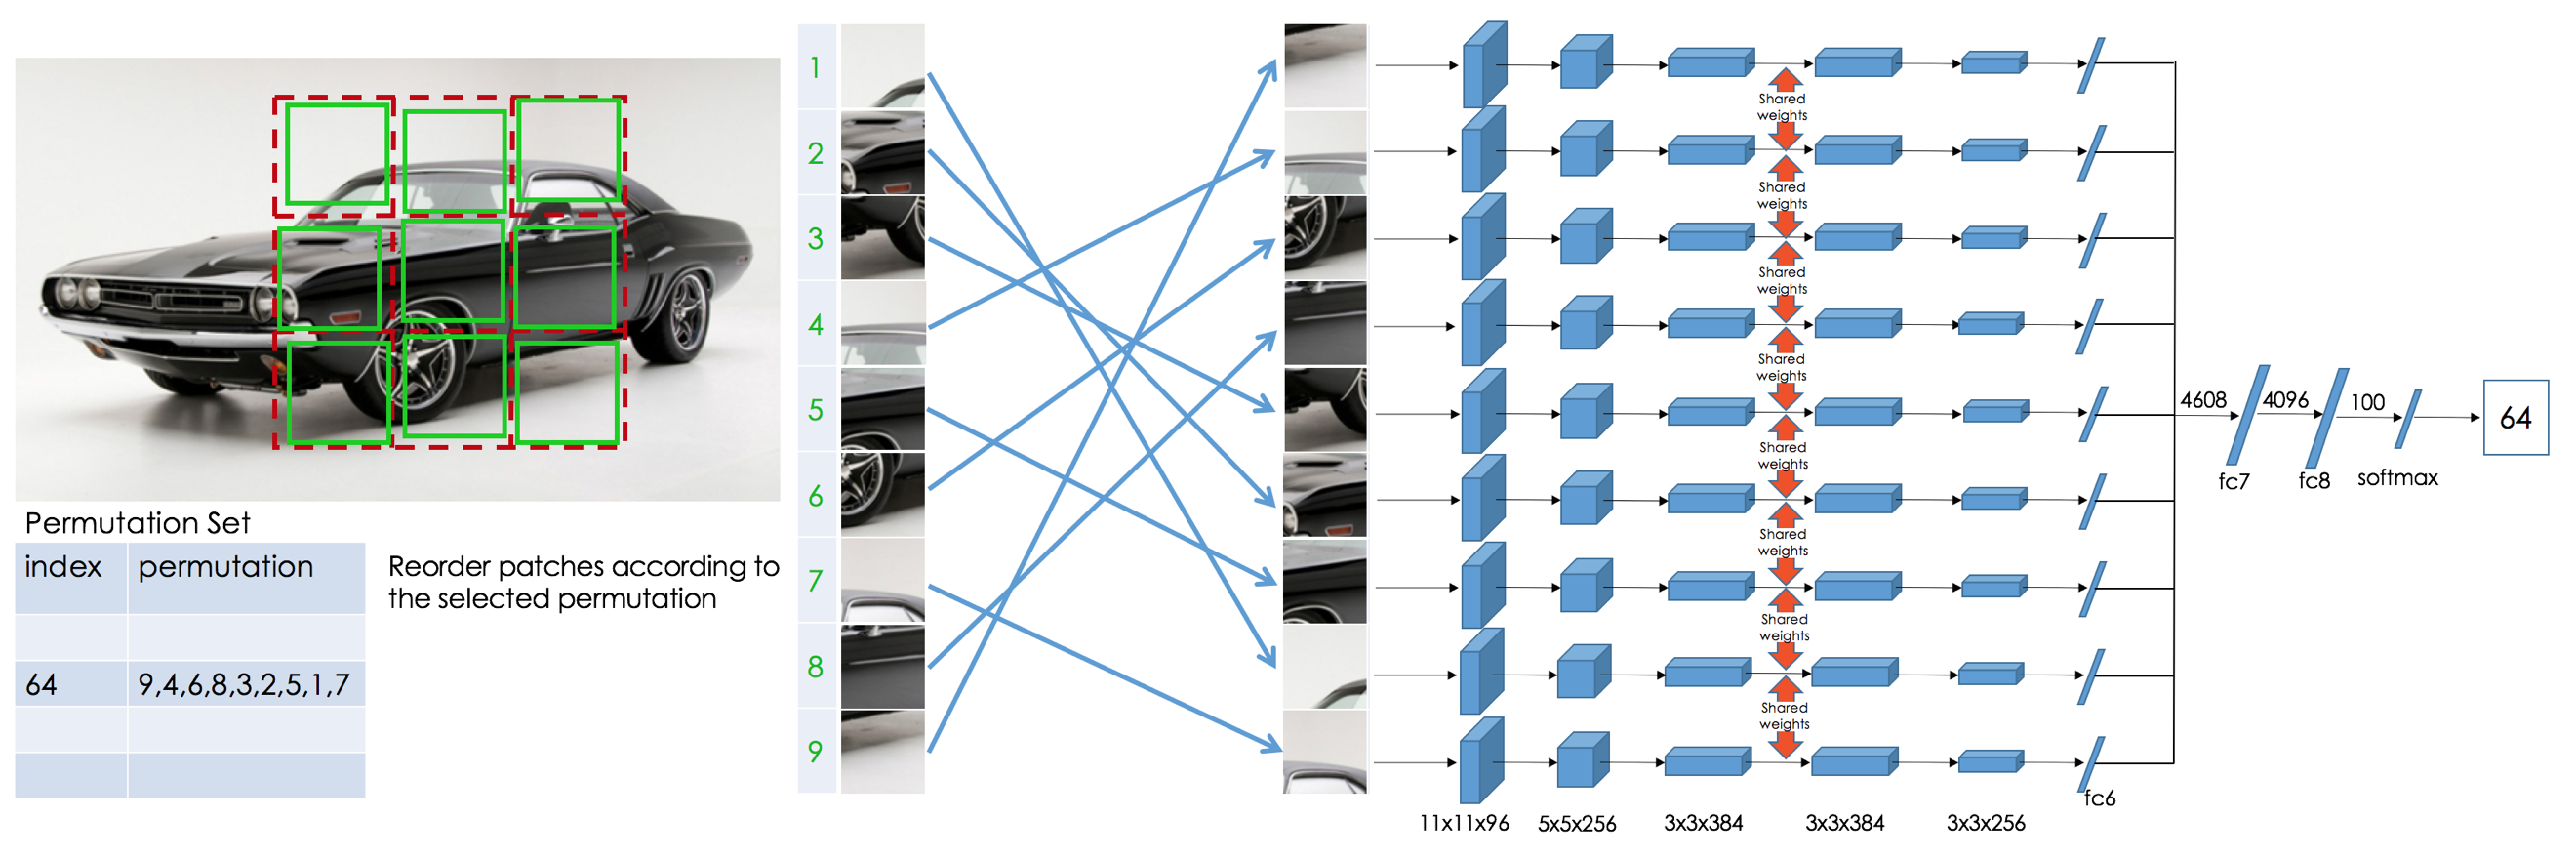
\includegraphics[width=\textwidth]{arquitectura_cfn}
	\caption{Arquitectura de Context-Free Network}
	\label{fig:arquitectura_cfn}
\end{figure}

Este modelo, mostrado en la Figura \ref{fig:arquitectura_cfn}, fue entrenado tomando 1.3M de imágenes del conjunto ImageNet, recortándolas en un \textit{grid} 3x3, permutando las nueve piezas resultantes y pasándoselas a la red junto con el orden correcto de las piezas, a modo de etiqueta. Partiremos de esta red convolucional ya entrenada por los autores y realizaremos sobre ella ligeras modificaciones.




\newpage
\section{Framework usado en el proyecto}

Hemos decidido usar \codeword{Caffe} (\codeword{pyCaffe}, en particular) como framework para el desarrollo de nuestro proyecto, el mismo que usan los autores del artículo y el modelo que usamos como base. En su \href{https://www.cvg.unibe.ch/media/project/noroozi/JigsawPuzzleSolver.html}{página oficial}, podemos encontrar tanto los pesos de su red CFN en un archivo con extensión \textbf{.caffemodel} como la arquitectura de la misma en un archivo \textbf{.prototxt}. En su \href{https://github.com/MehdiNoroozi/JigsawPuzzleSolver}{repositorio de Github} encontramos los ficheros prototxt usados para el entrenamiento de la red.

\codeword{Caffe} permite definir ficheros con el diseño del modelo y con los parámetros del proceso de compilación (en \codeword{Caffe}, realizado por un \textit{solver}). A partir de los ficheros con el diseño del modelo, es posible cargar los pesos preentrenados que se deseen, simplemente llamando a la capa del nuevo modelo con el mismo nombre de la capa cuyos pesos se quieran importar. \codeword{Caffe} también incluye distintos tipos de políticas de variación del ratio de aprendizaje con las que se han experimentado, en particular con el decaimiento \textbf{exponencial} y en \textbf{escalera} (más sobre esto en la sección siguiente). 

Este \textit{framework} no incluye opciones para especificar un criterio de parada, a parte de un número máximo de iteraciones. Para evitar un posible \textit{overfitting} en el entrenamiento, hemos implementado el \textit{early stopping} manualmente, que realizamos pasando cada \textit{batch} a la red, de uno en uno, monitorizando la \textbf{pérdida de validación media de cada época} y deteniendo el entrenamiento cuando esta aumenta (o cuando no decrece significativamente) durante cierto número de épocas.

\codeword{Caffe}, al igual que \codeword{Keras} y \codeword{TensorFlow}, admite soporte para cómputo en GPU, que se ha aprovechado en este proyecto. El código implementado se ha ejecutado en Google Colab y en el hardware personal de los autores de este proyecto. Sus especificaciones se muestran en la Figura \ref{fig:hardware_pc}.

\hfill \break


\begin{figure}[h]
	\centering
	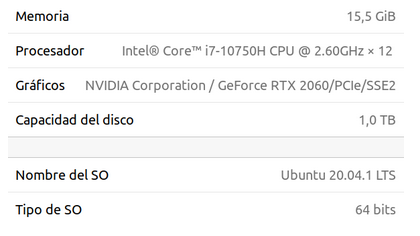
\includegraphics[width=300px]{hardware_pc}
	\caption{Hardware personal de los autores}
	\label{fig:hardware_pc}
\end{figure}







\newpage
\section{Ajuste fino sobre CIFAR100}

Nuestro primer experimento consistirá en tomar una de las ramas de la red CFN y adaptarla para resolver el problema de clasificación de CIFAR100 aplicándole un ajuste fino (\textit{fine tuning}). 

En lo que respecta al conjunto de datos utilizado, CIFAR100 cuenta con 100 clases distintas, cada una con 600 imágenes a color (500 para entrenamiento, 100 para test) de 32x32 píxeles de tamaño. Este dataset ha sido importado directamente desde los conjuntos de muestra que ofrece \codeword{Keras}, en forma de array de \codeword{numpy}. 

A nivel de arquitectura, lo único que cambia es que se eliminan las capas \textit{ReLU} y \textit{Dropout} tras la capa densamente conectada, esta se cambia por otra con 100 nodos (uno por cada clase) y se añade un clasificador \textit{softmax} al final de lo que antes era la rama de la red CFN. El resto de capas densamente conectadas, al final del modelo original, se eliminan para este entrenamiento supervisado. El diseño del modelo puede apreciarse en la Figura \ref{fig:arquitectura_sc}.

\begin{figure}[h]
	\centering
	\begin{subfigure}{\textwidth}
		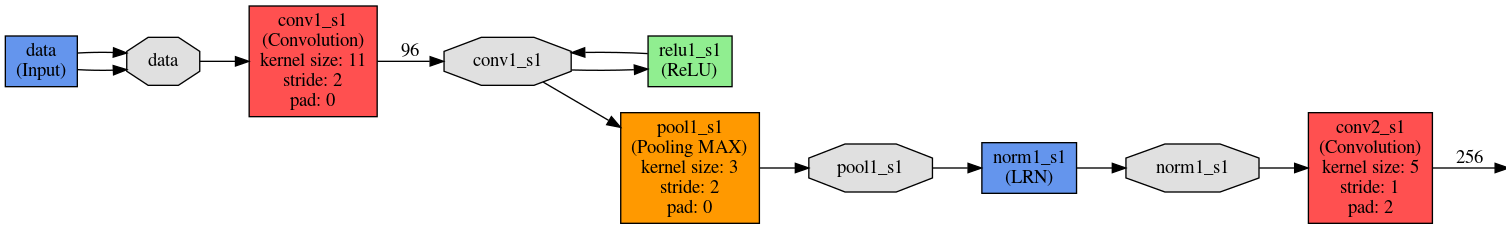
\includegraphics[width=\textwidth]{sc_model1}
	\end{subfigure}
	\begin{subfigure}{0.8\textwidth}
		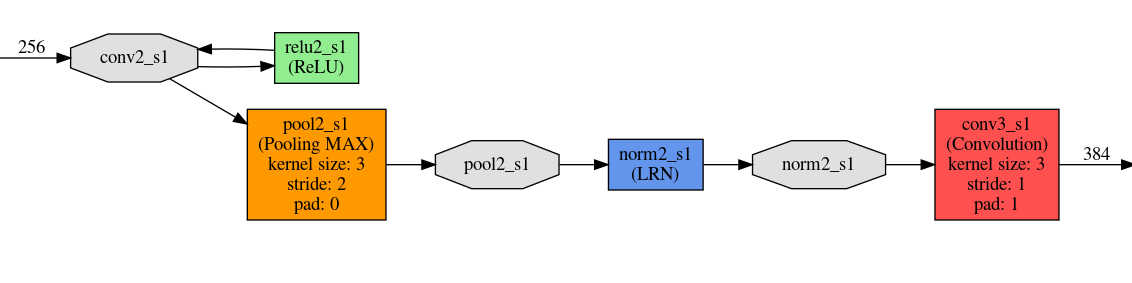
\includegraphics[width=\textwidth]{sc_model2}
	\end{subfigure}
	\begin{subfigure}{0.6\textwidth}
		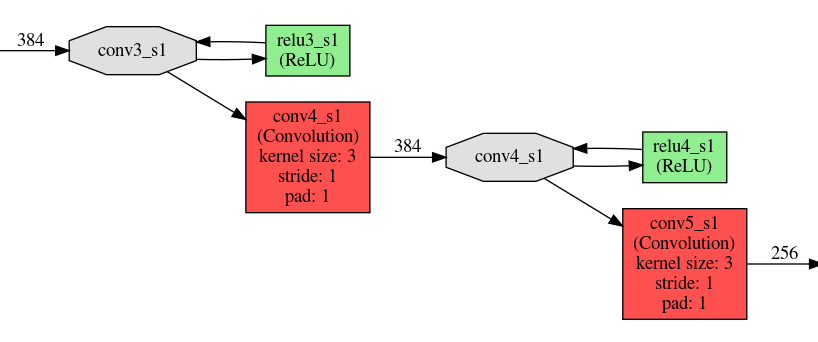
\includegraphics[width=\textwidth]{sc_model3}
	\end{subfigure}
	\begin{subfigure}{0.9\textwidth}
		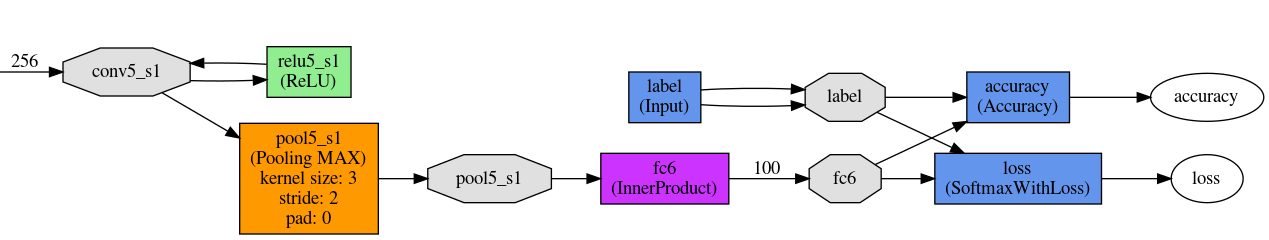
\includegraphics[width=\textwidth]{sc_model4}
	\end{subfigure}
	\caption{Arquitectura de nuestra red}
	\label{fig:arquitectura_sc}
\end{figure}



\subsection{Preprocesamiento de las imágenes}

En primer lugar, aplicamos un preprocesamiento sobre las imágenes de los conjuntos de entrenamiento y de test redimensionándolas a un tamaño de 64x64 (el utilizado como entrada de las imágenes en cada rama del modelo original) y normalizándolas. Esta normalización se ha llevado a cabo hallando la media y la desviación típica de los píxeles de todas las imágenes de entrenamiento en cada uno de sus canales. A continuación, para cada imagen normalizamos cada uno de sus canales restando por la media total en ese canal y dividiendo por su desviación típica. Para el preprocesado del conjunto de test se han aplicado la media y la desviación típica del conjunto de entrenamiento.


\subsection{Entrenamiento de la última capa}

Antes de realizar un ajuste fino es necesario entrenar la nueva capa de salida fijando los pesos de las capas previas, tal como indica \href{http://faculty.neu.edu.cn/yury/AAI/Textbook/Deep\%20Learning\%20with\%20Python.pdf}{aquí} (capítulo 5.3.2 Fine-tuning, pág. 154), para evitar una propagación del error desmedida generada en la última capa que perjudique a los pesos pre entrenados.  

Para realizar el entrenamiento, hemos decidido fijar un número máximo de 200 épocas y separar un 15\% de las imágenes del conjunto de entrenamiento para usarlas como conjunto de validación. El tamaño de lote aplicado en el entrenamiento original fue de 256, pero se ha reducido a 128 para mejorar la regularización, siguiendo las indicaciones dadas \href{https://arxiv.org/abs/1206.5533}{aquí}, aunque conservando un tamaño de lote lo suficientemente alto como para aprovechar el procesamiento paralelo de la GPU. 

Para poder entrenar la capa de salida previa al \textit{softmax}, (\textit{fc6}), esta se inicializa usando el método de Xavier Glorot uniforme, siguiendo las indicaciones de este \href{http://proceedings.mlr.press/v9/glorot10a.html}{artículo}, a diferencia de la inicialización gaussiana usada en el entrenamiento original. El resto de pesos de la red se mantienen congelados, como ya se ha explicado.

Además, con el objetivo de evitar un posible sobreajuste, aplicamos un \textit{early stopping} con \textit{patience} igual a 5. Hemos considerado que esta paciencia era adecuada teniendo en cuenta la política de aprendizaje utilizada (exponencial), puesto que es suficientemente alta para tolerar perturbaciones al principio del entrenamiento debidas a un \textit{learning rate} demasiado alto, pero también lo suficientemente baja para detener el entrenamiento cuando nos alejemos de un mínimo razonablemente bueno. A su vez, se ha añadido al criterio de parada que el entrenamiento se detenga no solamente cuando la pérdida de validación no mejore, sino también cuando esta baje menos de un $\epsilon = 10^{-4}$ durante un número de épocas que supere a la paciencia anterior.

El método de optimización utilizado ha sido Adam, por sus buenos resultados generales (como se indica en este \href{https://arxiv.org/pdf/1609.04747.pdf}{artículo}). Como esta capa va a ser entrenada desde cero, hemos decidido fijar un \textit{learning rate} de partida igual a 0.01, relativamente alto, que disminuye exponencialmente multiplicándose por una constante \textit{gamma} igual a 0.9995 después de cada iteración (aprendizaje sobre 1 batch). Considerando que el conjunto de entrenamiento tiene 42500 imágenes y que el tamaño de lote es de 128, esto equivale a multiplicar el ratio de aprendizaje por 0.85, aproximadamente, después de cada época.  También hemos fijado un \textit{weight decay} igual a 0.001, superior al de 0.0005 usado en el entrenamiento original, para favorecer la regularización.

El entrenamiento ha durado 64 épocas. En la Figura \ref{fig:loss_cifar} se muestra una gráfica con la evolución de la función de pérdida en entrenamiento y validación a lo largo del entrenamiento. Observamos un pico en las dos primeras iteraciones, probablemente a causa del error generado por la capa recién inicializada. Vemos que rápidamente la capa añadida empieza a aprender y las pérdidas de entrenamiento y validación comienzan a bajar.

\begin{figure}[h]
	\centering
	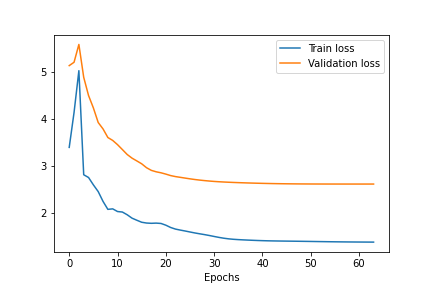
\includegraphics[width=0.6\textwidth]{loss_cifar}
	\caption{Evolución de la función de pérdida en entrenamiento y validación a lo largo del entrenamiento}
	\label{fig:loss_cifar}
\end{figure}

Después de evaluar el modelo con la última capa ya entrenada, hemos obtenido una precisión del 37.66\%.



\subsection{Ajuste fino}

Después de haber entrenado la última capa, intentaremos aplicar un ajuste fino para mejorar los resultados de nuestra red. Para ello, aunque hemos vuelto a utilizar Adam como optimizador en el ajuste fino, hemos decidido aplicar ligeros cambios a la política de entrenamiento que se ha seguido anteriormente. 

Por un lado, hemos bajado la paciencia establecida en \textit{early stopping} a 1 ya que el número de épocas invertidas para entrenar el modelo debe ser muy bajo (un máximo establecido de 50). Para evitar que los pesos cambien de forma drástica, se ha fijado un \textit{learning rate} base igual a 0.0005 que disminuye con una política en escalera, cuando se avanza un número de épocas prefijado, el \textit{learning rate} es multiplicado por un \textit{gamma} igual a 0.2. El valor de \textit{weight decay} también lo hemos bajado a 0.0005. Como apoyo a la visualización de las políticas aplicadas al ratio de aprendizaje, tanto para este entrenamiento como para el del apartado anterior, la gráfica de la Figura \ref{fig:lr_policies} representa la evolución de ambos \textit{learning rates}.

\begin{figure}[h]
	\centering
	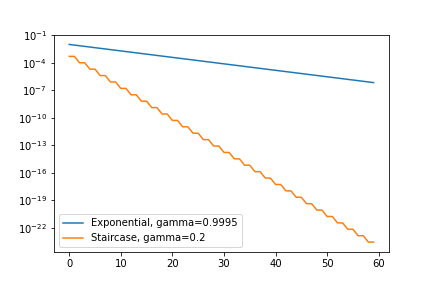
\includegraphics[width=0.6\textwidth]{lr_policies}
	\caption{Evolución de políticas de \textit{learning rates} aplicadas en el entrenamiento de la última capa y el ajuste fino. Nótese que la escala es logarítmica y que el ajuste fino se detiene en solamente 16 épocas aplicando el criterio de parada.}
	\label{fig:lr_policies}
\end{figure}


El entrenamiento ha durado 15 épocas. La gráfica de la Figura \ref{fig:loss_cifar_ft} muestra la evolución de las funciones de pérdida en entrenamiento y validación a lo largo del ajuste fino. 


\begin{figure}[h]
	\centering
	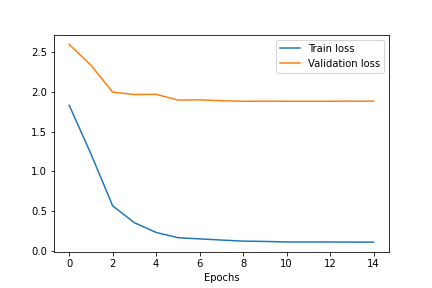
\includegraphics[width=0.6\textwidth]{loss_cifar_ft}
	\caption{Evolución de las pérdidas asociadas a los conjuntos de entrenamiento y validación durante el ajuste fino}
	\label{fig:loss_cifar_ft}
\end{figure}


En este caso, la evaluación del modelo ha devuelto una precisión del 52.7\%, una notable mejoría con respecto a los resultados anteriores al \textit{fine tuning}.





\subsection{Filtros aprendidos}

Como la red preentrenada que ajustamos ha sido entrenada de formas distintas a la habitual, nos interesa comprobar si la información que contiene es parecida a la de una red entrenada para clasificación. Hemos visualizado los filtros aprendidos en la primera capa convolucional que, como se indica en este \href{https://arxiv.org/abs/1411.1792}{artículo}, se destina al reconocimiento de patrones geométricos y fotométricos básicos. Esto se muestra en la Figura \ref{fig:filtros_cfn_vs_alexnet}, en la que podemos ver que algunos de los patrones que registran ambos conjuntos de filtros son parecidos, por ejemplo aquellos cuya forma consiste en varias bandas paralelas. Por otro lado, hay otros que solo aparecen en una de las dos redes, como aquellos que tienen forma circular, que solo aparecen en AlexNet. En general, parece que los filtros de la primera capa convolucional de la CFN son capaces de discernir patrones sencillos.

\begin{figure}[h]
	\begin{subfigure}{0.5\textwidth}
		\centering
		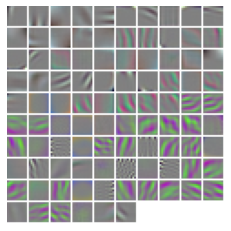
\includegraphics[height=160px,width=160px]{filtros_conv1_sc}
	\end{subfigure}
	\begin{subfigure}{0.5\textwidth}
		\centering
		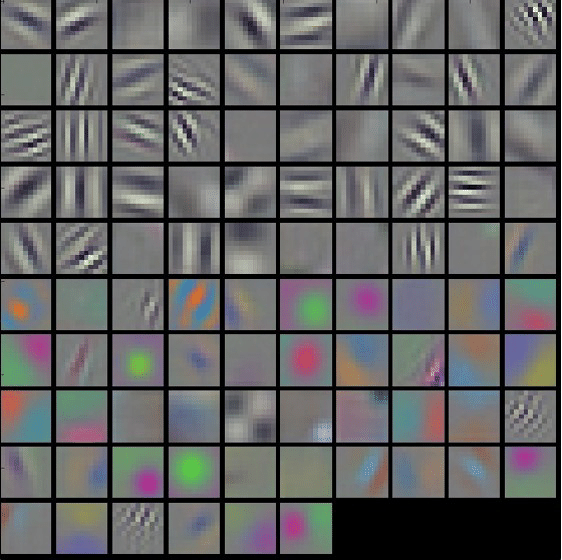
\includegraphics[height=150px,width=150px]{filtros_conv1_alexnet}
	\end{subfigure}
	\caption{Comparativa de los filtros aprendidos en la primera capa convolucional (destinada a la detección de patrones simples) por la CFN (a la izquierda) y por una AlexNet estándar (a la derecha).}
	\label{fig:filtros_cfn_vs_alexnet}
\end{figure}

También hemos comparado los mismos filtros de la CFN con los filtros obtenidos por nuestra red después del ajuste fino. Como se puede apreciar en la Figura \ref{fig:filtros_cfn_vs_sc_ft}, los filtros apenas cambian después de llevar a cabo el ajuste fino, lo cual es algo esperable pues esta técnica no pretende modificar los pesos de la red de forma drástica.

\begin{figure}[h]
	\begin{subfigure}{0.5\textwidth}
		\centering
		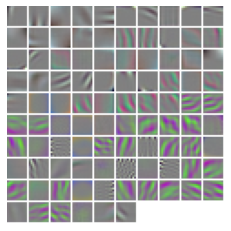
\includegraphics[height=160px,width=160px]{filtros_conv1_sc}
	\end{subfigure}
	\begin{subfigure}{0.5\textwidth}
		\centering
		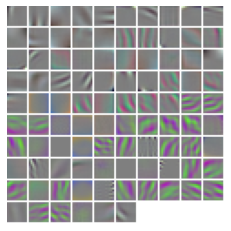
\includegraphics[height=160px,width=160px]{filtros_conv1_sc_ft}
	\end{subfigure}
	\caption{Comparativa de los filtros aprendidos en la primera capa convolucional por la CFN (a la izquierda) y por nuestra red después de realizar el ajuste fino (a la derecha).}
	\label{fig:filtros_cfn_vs_sc_ft}
\end{figure}



\subsection{Comparación con AlexNet}

Es clave recordar que la red pre entrenada utilizada para este experimento se basa en AlexNet y ha sido entrenada de forma autosupervisada, es decir, nuestro objetivo es acercarnos a los resultados obtenidos por AlexNet sobre el conjunto CIFAR100 entrenada desde cero y de forma supervisada para clasificar dicho conjunto de datos. 

Por un lado, la CFN comparte los mismos pesos en todas sus ramas, lo que reduce el número de parámetros de este modelo con respecto al de AlexNet, como se indica en su artículo correspondiente, de los 61M parámetros de AlexNet a solamente 27.5M parámetros. La estructura en ramas de la CFN es necesaria para la extracción de características de todas las partes de una imagen para aprender a resolver los puzzles, pero el menor número de parámetros además permite un aprendizaje más rápido.

Por otro lado, de acuerdo con este \href{https://www.researchgate.net/publication/301835547_Network_of_Experts_for_Large-Scale_Image_Categorization}{artículo} en el que se muestran, entre otras cosas, los resultados de AlexNetC100 (AlexNet entrenada con CIFAR100), esta red consigue en torno a un 54\% de precisión.

Si comparamos estos resultados con los obtenidos a partir de la red entrenada de forma autosupervisada, vemos que nuestro error en test es ligeramente mayor (un 1.3\%), pero teniendo en cuenta la desventaja del modelo del que partimos (falta de anotaciones y entrenamiento a partir de imágenes de un conjunto de datos distinto) consideramos que nuestros resultado son positivos en favor del aprendizaje autosupervisado con la resolución de puzzles como pretexto.






\newpage
\section{Ajuste fino sobre FRUITS360}

El conjunto CIFAR100 es un dataset variado y relativamente complejo. Los resultados obtenidos en el experimento anterior son relativamente buenos si los comparamos con los de AlexNet, pero un error del 47.3\% no ofrece garantías en un problema real. Como complemento al experimento anterior, hemos probado a repetirlo con la misma red (una rama de la CFN) con otro conjunto de datos, Fruits360, que contiene imágenes de un gran número de frutas, cada una desde distintos ángulos.

\subsection{Preprocesamiento de las imágenes}

Este conjunto de datos contiene más de 90000 imágenes, que no ha sido posible preprocesar conjuntamente  debido a las limitaciones de memoria RAM y de velocidad de flujo de datos en Colab. Por tanto, hemos tomado la decisión de reducir el conjunto de entrenamiento a una cuarta parte, lo cual no debería suponer un perjuicio a la validez del experimento debido al enorme parecido entre muchas de las imágenes, que corresponden a la misma fruta desde ángulos muy cercanos. En la Figura \ref{fig:apple_golden_train} tomamos una pequeña muestra de las 8 primeras imágenes correspondientes a la clase \textit{Apple Golden} en el conjunto de entrenamiento.

\begin{figure}[h]
	\begin{subfigure}{0.24\textwidth}
		\centering
		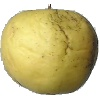
\includegraphics[height=60px,width=60px]{apple_golden_train0}
	\end{subfigure}
	\begin{subfigure}{0.24\textwidth}
		\centering
		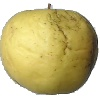
\includegraphics[height=60px,width=60px]{apple_golden_train1}
	\end{subfigure}
	\begin{subfigure}{0.24\textwidth}
		\centering
		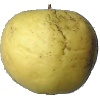
\includegraphics[height=60px,width=60px]{apple_golden_train2}
	\end{subfigure}
	\begin{subfigure}{0.24\textwidth}
		\centering
		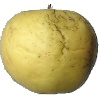
\includegraphics[height=60px,width=60px]{apple_golden_train3}
	\end{subfigure}
	\begin{subfigure}{0.24\textwidth}
		\centering
		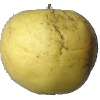
\includegraphics[height=60px,width=60px]{apple_golden_train4}
	\end{subfigure}
	\begin{subfigure}{0.24\textwidth}
		\centering
		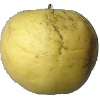
\includegraphics[height=60px,width=60px]{apple_golden_train5}
	\end{subfigure}
	\begin{subfigure}{0.24\textwidth}
		\centering
		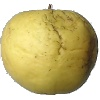
\includegraphics[height=60px,width=60px]{apple_golden_train6}
	\end{subfigure}
	\begin{subfigure}{0.24\textwidth}
		\centering
		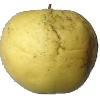
\includegraphics[height=60px,width=60px]{apple_golden_train7}
	\end{subfigure}
	\caption{Muestra de las 8 primeras imágenes de la clase \textit{Apple Golden} en el conjunto de entrenamiento}
	\label{fig:apple_golden_train}
\end{figure}


La criba se ha realizado recorriendo los directorios que se encuentran dentro del directorio de entrenamiento del dataset (uno por cada clase) y leyendo solamente 1 de cada 4 imágenes. También se ha reducido el número de frutas, de 131 clases de frutas distintas a 81 clases. Cada imagen ha sido redimensionada a 64x64 píxeles, buscando que la red aproveche sus pesos aprendidos para extracción de características de forma óptima. Las imágenes se barajan y, como en el experimento anterior, un 15\% de las imágenes del conjunto de entrenamiento se separa y se destina a validación.

\subsection{Entrenamiento de la última capa}

Las condiciones del entrenamiento para la capa de salida, con el resto de la red congelada, han sido las mismas que en el análogo para CIFAR100, salvo por la necesidad de cambiar la capa densa de salida a una con 81 nodos en correspondencia con el número de clases. El entrenamiento ha concluido en 98 épocas y la evolución de la función de pérdida puede verse en la Figura \ref{fig:loss_fruits}. La precisión en la fase de test es un 91\%.

\begin{figure}[h]
	\centering
	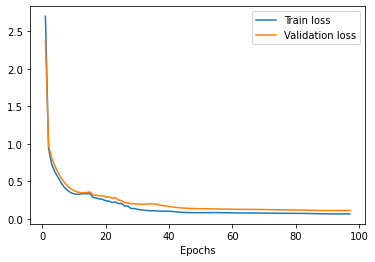
\includegraphics[width=0.6\textwidth]{loss_fruits}
	\caption{Evolución de las pérdidas asociadas a los conjuntos de entrenamiento y validación durante el entrenamiento de la última capa}
	\label{fig:loss_fruits}
\end{figure}


\subsection{Ajuste fino}

Para el \textit{fine tuning}, a partir de los pesos obtenidos del entrenamiento anterior para la última capa, sí se han modificado ligeramente los hiperparámetros. A raíz de los mejores resultados obtenidos en la fase anterior, se ha considerado que los resultados obtenidos eran relativamente buenos y que podría merecer la pena reducir el ratio de aprendizaje inicial, de 0.0005 a 0.0003, para evitar que la red pueda salir de un óptimo local. El valor del \textit{stepsize} (número de lotes procesados por la red antes de la reducción del \textit{learning rate}) se ha aumentado para tener en cuenta el mayor número de batches en este conjunto de datos (el tamaño de \textit{batch} se ha dejado igual que en experimento con CIFAR100). 

El entrenamiento ha durado 15 épocas y las funciones de pérdida de entrenamiento y validación han evolucionado según se muestra en la Figura \ref{fig:loss_fruits_ft}. La precisión obtenida en la fase de prueba ha sido del 96.91\% que, a pesar de la reducción del número de clases y de la criba que se realiza posteriormente en el conjunto de entrenamiento, son resultados bastante buenos en términos generales.

\begin{figure}[h]
	\centering
	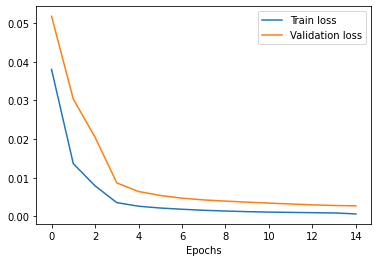
\includegraphics[width=0.6\textwidth]{loss_fruits_ft}
	\caption{Evolución de las pérdidas asociadas a los conjuntos de entrenamiento y validación durante el ajuste fino}
	\label{fig:loss_fruits_ft}
\end{figure}








\newpage
\section{Conclusiones}

En esta práctica hemos realizado una serie de experimentos a partir de un modelo basado en AlexNet, pre entrenado de forma auto supervisada usando como pretexto la resolución de puzzles a partir de imágenes de ImageNet. En particular, hemos adaptado el modelo a dos datasets diferentes, CIFAR100 y una versión reducida de Fruits360 con 81 clases, y hemos realizado un ajuste fino del modelo sobre ambos.

Consideramos que los resultados alcanzados han sido buenos en los dos casos. Para el conjunto CIFAR100, hemos obtenido una precisión del 52.7\% después del ajuste fino, considerablemente cercano al 54\% de precisión que obtiene AlexNet entrenado totalmente a partir de este conjunto de datos de forma supervisada. Para el conjunto Fruits360 reducido, hemos logrado un error ligeramente por encima del 3\%, lo que es un éxito en términos generales.

En conclusión, consideramos que los experimentos realizados suponen un argumento para el entrenamiento de CNNs mediante el pretexto de la resolución de puzzles, suponiendo esta una alternativa al aprendizaje supervisado que requiere de conjuntos de datos de gran tamaño etiquetados manualmente.




\newpage
\section{Bibliografía}

\begin{enumerate}
	\item \href{https://www.fast.ai/2020/01/13/self_supervised/}{Self-supervised learning and computer vision }
	\item \href{https://www.cvg.unibe.ch/media/project/noroozi/JigsawPuzzleSolver.html}{Unsupervised Learning of Visual Representations by Solving Jigsaw Puzzles (project)}
	\item \href{https://github.com/MehdiNoroozi/JigsawPuzzleSolver}{Unsupervised Learning of Visual Representations by Solving Jigsaw Puzzles (repositorio de Github)}
	\item \href{https://arxiv.org/pdf/1603.09246v3.pdf}{Unsupervised Learning of Visual Representations by Solving Jigsaw Puzzles (paper)}
	\item \href{https://recodeminds.com/blog/a-beginners-guide-to-caffe-for-deep-learning/}{Beginner's guide to Caffe}
	\item \href{https://github.com/BVLC/caffe/blob/master/examples/02-fine-tuning.ipynb}{Fine-tuning a Pretrained Network for Style Recognition}
	\item \href{http://faculty.neu.edu.cn/yury/AAI/Textbook/Deep\%20Learning\%20with\%20Python.pdf}{Deep Learning with Python}
	\item \href{https://arxiv.org/abs/1206.5533}{Practical recommendations for gradient-based training of deep architectures}
	\item \href{http://proceedings.mlr.press/v9/glorot10a.html}{Understanding the difficulty of training deep feedforward neural networks}
	\item \href{https://arxiv.org/pdf/1609.04747.pdf}{An overview of gradient descent optimization algorithms}
	\item \href{https://arxiv.org/abs/1411.1792}{How transferable are features in deep neural networks?}
	\item \href{https://github.com/arundasan91/Deep-Learning-with-Caffe/blob/master/Deep-Neural-Network-with-Caffe/Deep\%20Neural\%20Network\%20with\%20Caffe.md}{Deep Neural Network with Caffe}
	\item \href{https://www.researchgate.net/publication/301835547_Network_of_Experts_for_Large-Scale_Image_Categorization}{Network of Experts for Large-Scale Image Categorization}
	\item \href{https://www.kaggle.com/moltean/fruits}{Fruits 360 dataset}
\end{enumerate}




















\end{document}



